\documentclass[11pt,letterpaper]{article}
\usepackage[utf8]{inputenc}
\usepackage[left=1in,right=1in,top=1in,bottom=1in]{geometry}
\usepackage{amsfonts,amsmath}
\usepackage{graphicx,float}
\usepackage{esint}
\usepackage{csquotes}
% -----------------------------------
\usepackage{hyperref}
\hypersetup{%
  colorlinks=true,
  linkcolor=blue,
  citecolor=blue,
  urlcolor=blue,
  linkbordercolor={0 0 1}
}
% -----------------------------------
\usepackage[authordate,backend=biber]{biblatex-chicago}
\addbibresource{citation.bib}
% -----------------------------------
\usepackage{fancyhdr}
\newcommand\course{MATH-UA.0230, PHYS-UA 180\\Introduction to Fluid Dynamics}
\newcommand\hwnumber{4}                  % <-- homework number
\newcommand\NetIDa{Ryan Sh\`iji\'e D\`u} 
\newcommand\NetIDb{February 23rd, 2023}
\pagestyle{fancyplain}
\headheight 35pt
\lhead{\NetIDa\\\NetIDb}
\chead{\textbf{\Large Worksheet \hwnumber}}
\rhead{\course}
\lfoot{}
\cfoot{}
\rfoot{\small\thepage}
\headsep 1.5em
% -----------------------------------
\usepackage{titlesec}
\renewcommand\thesubsection{(\arabic{section}.\alph{subsection})}
\titleformat{\subsection}[runin]
        {\normalfont\bfseries}
        {\thesubsection}% the label and number
        {0.5em}% space between label/number and subsection title
        {}% formatting commands applied just to subsection title
        []% punctuation or other commands following subsection title
% -----------------------------------
\setlength{\parindent}{0.0in}
\setlength{\parskip}{0.1in}
% -----------------------------------
\newcommand{\de}{\mathrm{d}}
\newcommand{\DD}{\mathrm{D}}
\newcommand{\pe}{\partial}
\newcommand{\mcal}{\mathcal}
%\newcommand{\pdx}{\left|\frac{\partial}{\partial_x}\right|}

\newcommand{\dsp}{\displaystyle}

\newcommand{\norm}[1]{\left\Vert #1 \right\Vert}
%\newcommand{\mean}[1]{\left\langle #1 \right\rangle}
\newcommand{\mean}[1]{\overline{#1}}
\newcommand{\inner}[2]{\left\langle #1,#2\right\rangle}

\newcommand{\ve}[1]{\boldsymbol{#1}}

\newcommand{\thus}{\Rightarrow \quad }
\newcommand{\fff}{\iff\quad}
\newcommand{\qdt}[1]{\quad \mbox{#1} \quad}

\renewcommand{\Re}{\mathrm{Re}}
\renewcommand{\Im}{\mathrm{Im}}
\newcommand{\E}{\mathbb{E}}
\newcommand{\lap} {\nabla^2}
\renewcommand{\div}{\nabla\cdot}

\newcommand{\csch}{\text{csch}}
\newcommand{\sech}{\text{sech}}


\newcommand{\hot}{\text{h.o.t.}}

\newcommand{\ssp}{\left.\qquad\right.}

\newcommand{\var}{\text{var}}
\newcommand{\cov}{\text{cov}}


\begin{document}

\section{Bernoulli's principle: examples}
\subsection{Flow out of a water tank}
Imagine a water tank with height $h$ of water inside. At the bottom there is a small hole. What would be the speed of the water flowing out of the hole.

\subsection{Venturi effect}
Calculate the fluid velocity difference at point 1 and 2 as a function of $h$.

Image from Wikipedia for Venturi effect. It is best to extend the lower end of the two vertical tubes to the center of the horizontal tube so that they stop at point 1 and 2.
\begin{figure}[H]
    \centering
    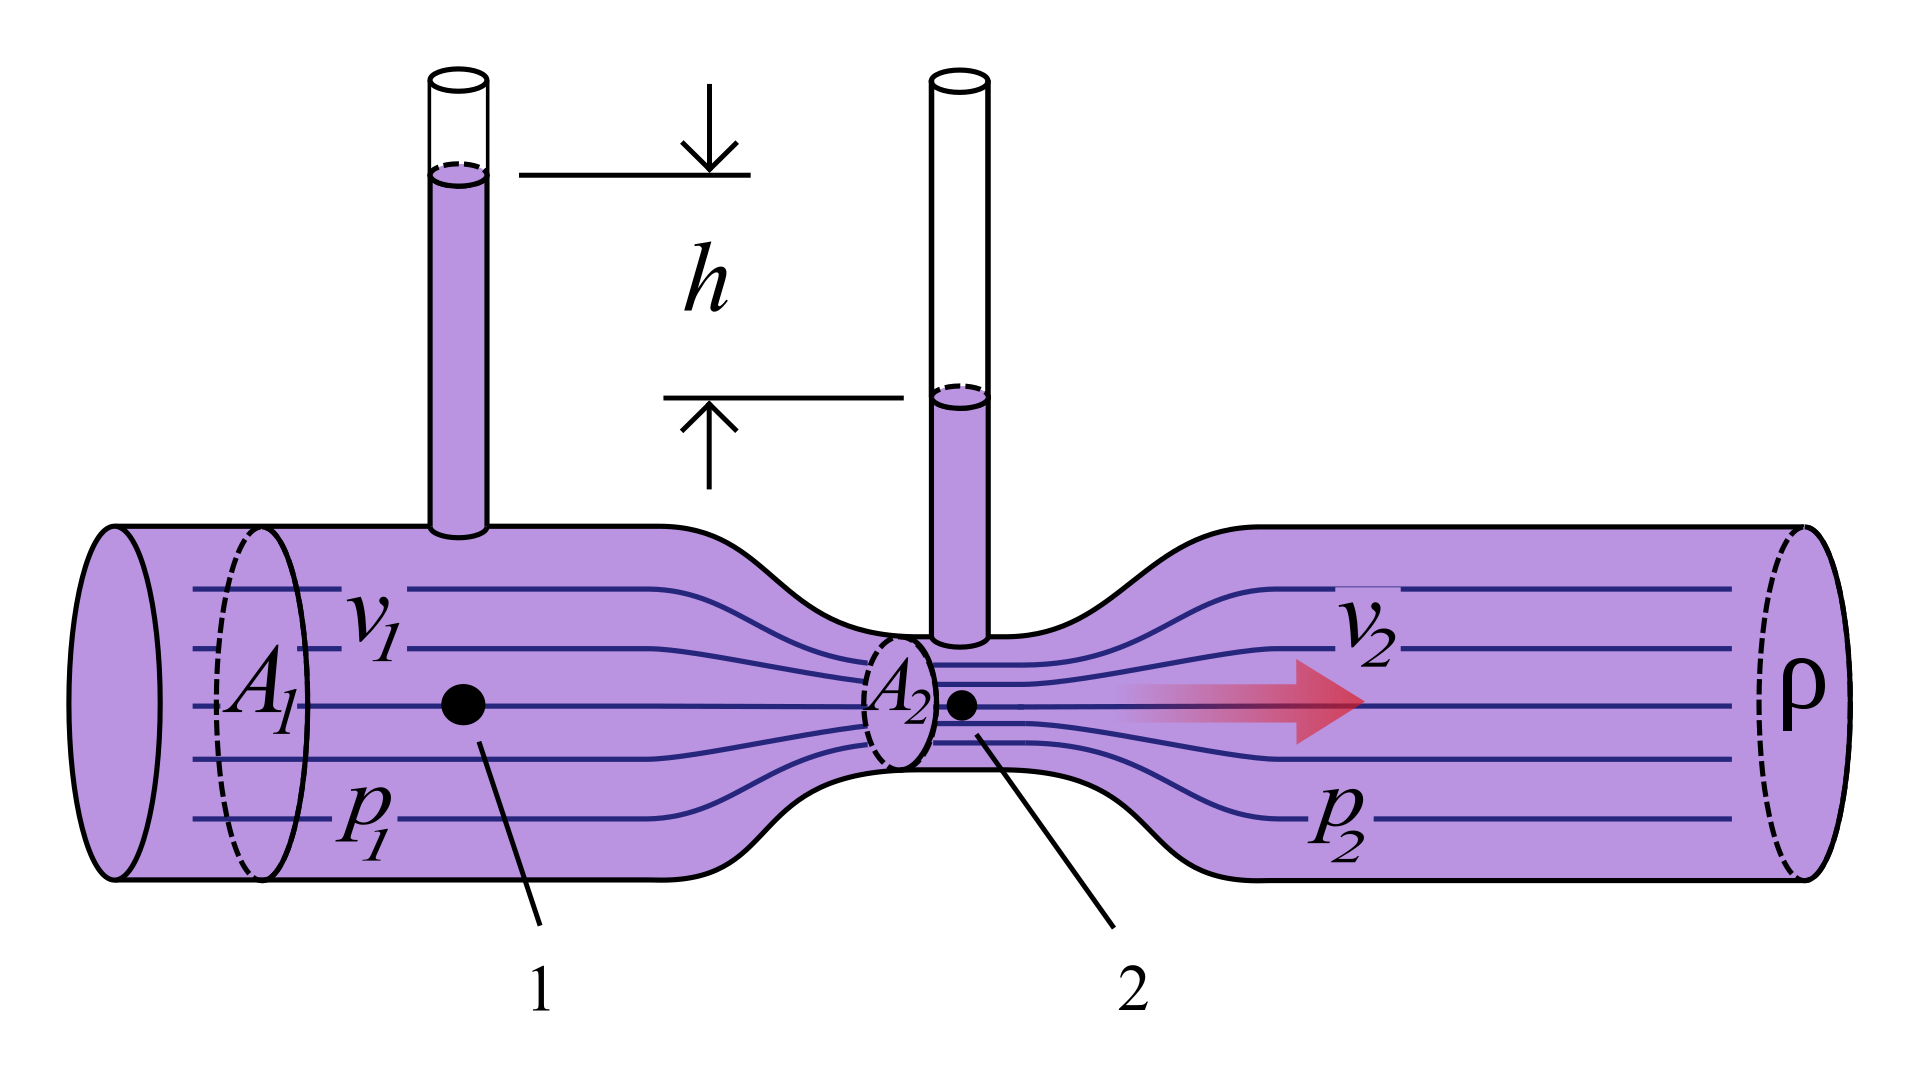
\includegraphics[width=0.5\textwidth]{figs/Venturi_wiki}
\end{figure}

\subsection{Pitot's tube}
Using the idea of the above device, think of a device that measures the speed of the fluid flow.

\subsection{Lift on an airfoil: a first look}
Use Bernoulli's principle to explain how lift is generated by a plane's wing.

Image generated by Wolfram software from \url{https://demonstrations.wolfram.com/JoukowskiAirfoilFlowField/}. The lines are streamlines, the color is the pressure field.
\begin{figure}[H]
    \centering
    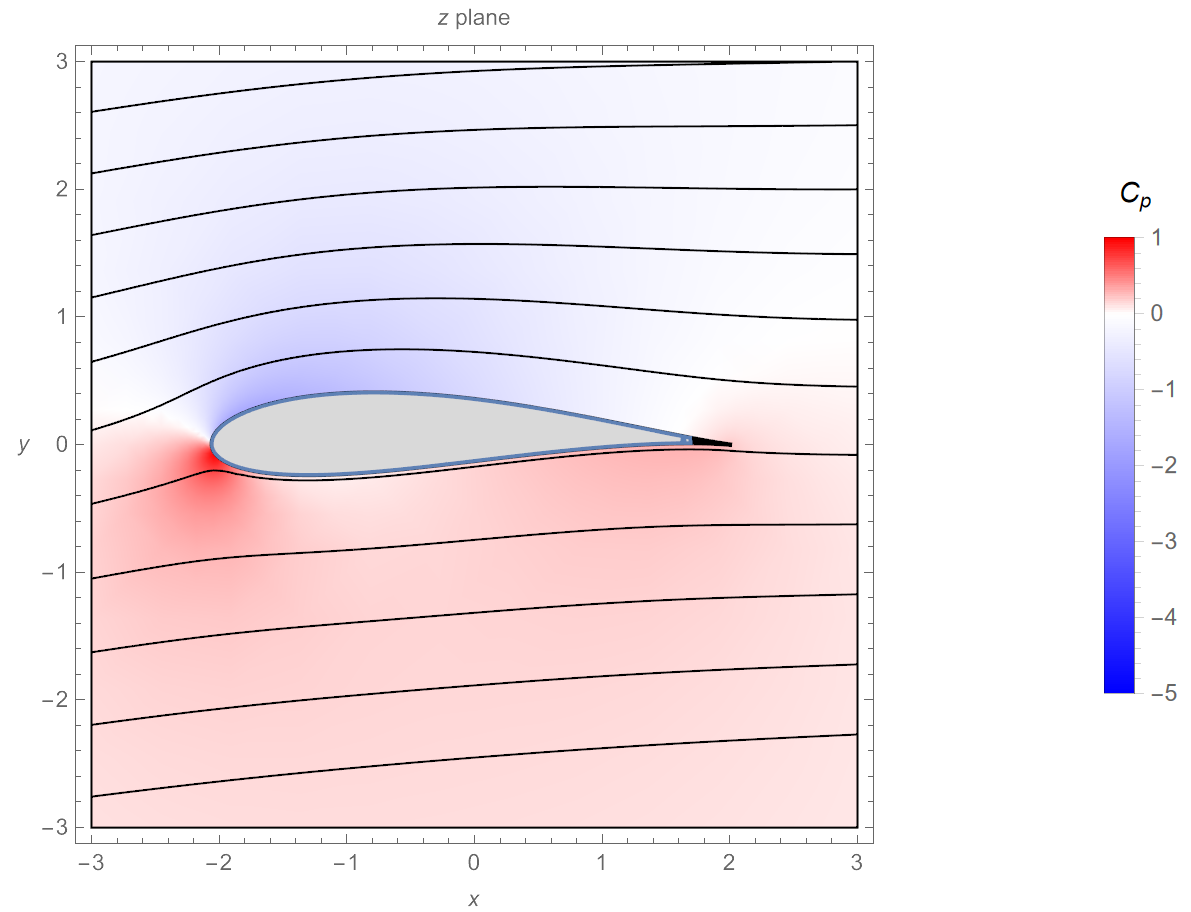
\includegraphics[width=0.6\textwidth]{figs/Airfoil}
\end{figure}



\section{Taylor–Green vortex}
The Taylor–Green vortex is an exact solution to the 2D Navier-Stokes equation:
\begin{align}
    &\frac{\partial u}{\partial t} + u\frac{\partial u}{\partial x} + v\frac{\partial u}{\partial y} = -\frac{1}{\rho} \frac{\partial p}{\partial x} + \nu \left( \frac{\partial^2 u}{\partial x^2} + \frac{\partial^2 u}{\partial y^2} \right),\\
    &\frac{\partial v}{\partial t} + u\frac{\partial v}{\partial x} + v\frac{\partial v}{\partial y} = -\frac{1}{\rho} \frac{\partial p}{\partial y} + \nu \left( \frac{\partial^2 v}{\partial x^2} + \frac{\partial^2 v}{\partial y^2} \right),\\
    &\frac{\partial u}{\partial x}+ \frac{\partial v}{\partial y} = 0.
\end{align}
The first appearance of this flow is in \cite{Taylor_23}. The name of this flows comes from the joint work \cite{TaylorGreen_37}. A 3D extension of the Taylor–Green vortex appeared recently in \cite{Antuono_20}. The exact solutions to the fluid equations are important tools for benchmarking numerical solvers for fluids dynamics. 

\subsection{}
The Taylor–Green vortex has velocity
\begin{align}
    u &= \cos x\sin y F(t)\\
    v &= -\sin x\cos y F(t).
\end{align}
Show, by plugging the velocity into the momentum equation, that the pressure field is given by
\begin{align}
    p = -\frac{\rho}{4}(\cos 2x+\cos 2y)F^2(t).
\end{align}

\subsection{}
Now show that the time component is
\begin{align}
    F(t) = e^{-2\nu t}.
\end{align}

\section{Alternative form for momentum dissipation}
\subsection{}
[From \cite{Aris_62}, Exercise 3.24.5] Show the vector identity
\begin{align}
    \nabla^2 \ve v = \nabla(\nabla\cdot\ve v)-\nabla\times(\nabla\times \ve v).
\end{align}

\subsection{}
[From \cite{Aris_62}, \S 6.11] Show that the incompressible Navier-Stokes can alternatively be written as
\begin{align}
    \rho\frac{D\ve v}{Dt} &= -\nabla p-\mu\nabla\times\ve \omega.
\end{align}

\newpage
\section{Energy dissipation in Navier-Stokes}
\subsection{}
Show the vector identity
\begin{align}
    \nabla\cdot(\ve a\times\ve b) = (\nabla\times\ve a)\cdot\ve b-\ve a\cdot(\nabla\times\ve b).
\end{align}

\subsection{}
[From \cite{Aris_62}, Exercise 6.14.4] For an incompressible Newtonian fluid moving within a fixed stationary boundary with no body forces, show that the total rate of dissipation of kinetic energy is
\begin{align}
    -\mu \iiint_V \ve\omega^2 \;\de V.
\end{align}

\subsection{}
To get another form of the total rate of dissipation of kinetic energy, we can work with the dissipation in Navier-Stokes directly. Dot it with $\ve v$ and integrate over the domain, we have
\begin{align}
    \mu \iiint_V \ve v\nabla^2\ve v \;\de V &= -\mu \iiint_V \nabla \ve v:\nabla\ve v \;\de V.
\end{align}

\subsection{}
In lecture you learned the total rate of dissipation of kinetic energy is
\begin{align}
    -2\mu \iiint_V \ve E:\ve E \;\de V.
\end{align}
These three forms should all be equal. Make sense of this by assume 
\begin{align}
    \iiint_V \ve E:\ve E \;\de V = \iiint_V \ve W:\ve W \;\de V.\label{eq:EW_ident}
\end{align}
To show \eqref{eq:EW_ident}, do plenty of integration by parts and use incompressibility.




% \section{}
% [From \cite{Aris_62}, Exercise 6.11.1] 




    
\vfill
\printbibliography


\end{document}